\chapter[Formato do TCC]{Formato do TCC}
\label{cap:formatoTCC}

Este capítulo apresenta o formato padrão a ser utilizado no TCC baseado nas normas da ABNT e no modelo ABNTex2, que também segue tais normas~\cite{abntTxtAcad2011,abntex2modelo}. Um TCC está dividido em três partes:  (1) elementos pré-textuais em que se encontram elementos como, por exemplo, a capa, o sumário e a lista de ilustrações; (2)  elementos textuais, em que será apresentado o conteúdo textual dividido em capítulos;  (3) os conteúdos pós-textuais em que são apresentadas as referências bibliográficas, os apêndices e os anexos. Tais elementos serão descritos neste capítulo.


\section{Elementos Pré-textuais}
\label{sec:preTextual}

Conforme demonstrado no presente documento, os elementos pré-textuais contam com a contra-capa, a capa, a folha de aprovação, a dedicatória, os agradecimentos, a epígrafe, o resumo em português e em inglês (\textit{abstract}). Logo após, são apresentados a lista de ilustrações, as tabelas, a lista de abreviaturas e siglas, a lista de símbolos e, por fim, o sumário.
Dentre estes itens, são opcionais a dedicatória, os agradecimentos,  a epígrafe,  a lista de símbolos e a lista de abreviaturas e siglas. A ABNT não estabelece um tamanho fixo para o título de cada  elemento pré-textual (ex. agradecimento, resumo), porém, no presente documento,  utilizou-se a fonte \textit{Latin Modern Sans} tamanho 24pt. Quanto à paginação, os elementos pré-textuais não recebem numeração de páginas, porém serão contabilizados.


Na capa deverá constar o nome completo do autor no topo em fonte 14pt (tamanho sugerido pelo ABNTex2). Logo após, no meio desta página, é apresentado o título na fonte 20pt. No final da página é apresentado o local e o ano em que o TCC foi/será apresentado em fonte 14pt. Similarmente, na contra-capa, será apresentado o nome do autor no topo da página e, abaixo, é apresentado o título do trabalho. Em seguida, é apresentado o preâmbulo. 
Após o preâmbulo, apresenta-se o nome da instituição, departamento e curso, o nome do orientador e coorientador. Finalmente, no final da página, é apresentado o local  e ano em que o TCC foi/será apresentado. Na folha seguinte, na versão final de seu TCC, deverá ser anexada a folha de aprovação.


A dedicatória deverá ser colocada no centro da página, em itálico com a fonte 12pt. O verso desta página ficará em branco. Em seguida, são apresentados os agradecimentos que também é um item opcional, porém importante, principalmente se sua pesquisa obteve algum tipo de financiamento (CNPq, Fapemig, etc.).  Logo após, em uma outra folha~\footnote{Note que, como estamos mencionando folha, caso o agradecimento ocupe apenas uma página, a página seguinte ficará em branco.}, é apresentada a epígrafe no final da página, à direita.

Uma nova folha também será destinada ao resumo. No final do resumo, cria-se um novo parágrafo para apresentar as palavras chaves. A expressão "Palavras-chaves:" deverá aparecer em negrito e cada palavra-chave deverá ser separada por um ponto. Logo após, em uma nova folha, é apresentado o resumo em língua estrangeira com a mesma formatação do resumo.

Em seguida, apresenta-se a lista de ilustrações, as tabelas, as abreviaturas e siglas, os símbolos e o sumário. Lembre-se de começar cada uma dessas listas (e o sumário) em uma nova folha. Faça a formatação destas listas conforme apresentado neste documento. Para o sumário, sempre deixe o índice de cada capítulo/seção à esquerda, seguido do seu título e, à direita, o número da página. Colocar uma sequência de pontos "...." entre o nome e a página onde se encontra a determinada seção. 

%O nome do capítulo, apêndice e anexo deve ser sempre em maíuscula e, das seções, em com a letra de cada palavra em maiúscula (exceto preposições e artigos).

\section{Elementos Textuais}
\label{sec:textual}

Os elementos textuais são separados por capítulos e, em cada capítulo, diversas seções e subseções. A fonte do corpo do texto será de 12pt. A Figura \ref{fig:elementosMonografia} mostra um esquema com os principais elementos de uma monografia e suas relações.

\begin{figure}[htb!]
    \centering
    \caption{Principais elementos de uma monografia e suas relações}
    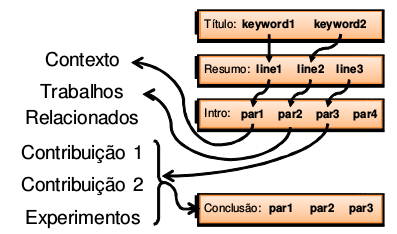
\includegraphics[keepaspectratio=true,scale=0.8]
    	{img/modelo_trabalho_academico.png}
    \legend{Fonte: \citeonline{mirelaTCC}.}
    \label{fig:elementosMonografia}
\end{figure}



Cada capítulo deve-se iniciar em uma nova folha. A ABNT não define um tamanho ou uma fonte específica para o título do capítulo e de suas seções. Neste documento, o título do capítulo e seu número foram apresentados na fonte \textit{Latin Modern Sans} de tamanho 24pt em negrito. 
As seções (seções de nível 1) foram apresentadas com a mesma fonte em negrito de tamanho 17pt, as subseções (seções de nível 2) de tamanho 14pt e, as seções de níveis 3 e 4, de tamanho 12pt. Observe, a seguir, exemplos de seções de níveis 2, 3 e 4.




\subsection{Exemplo de Seção de Nível 2}
\subsubsection{Exemplo de Seção de Nível 3}
\subsubsubsection{Exemplo de Seção de Nível 4}

Segundo a \citeonline{abntTxtAcad2011}, a numeração dos elementos textuais, quando utilizada apenas a frente da folha, deverá ser apresentada no canto direito superior. Quando, no TCC, utiliza-se a frente e o verso da folha, a frente deverá possuir a numeração no canto direito superior e, o verso, no canto esquerdo superior.

Seguindo as normas  \citeonline{ibge1993,abntTxtAcad2011}, conforme apresentado nas Figuras~\ref{fig:elementosMonografia} e \ref{fig:desenhoAutor}, cada ilustração deve possuir o seu título na parte superior e a fonte de onde foi retirada esta figura na parte inferior. É importante notar que é obrigatório colocar a fonte consultada, mesmo que esta seja o próprio autor. As tabelas devem ser apresentadas conforme a Tabela~\ref{tab:exemploTabela}. Caso queira mais exemplos de tabelas, conferir o padrão~\citeonline{ibge1993}. 

\begin{figure}[htb!]
    \centering
    \caption{Desenho feito pelo autor}
    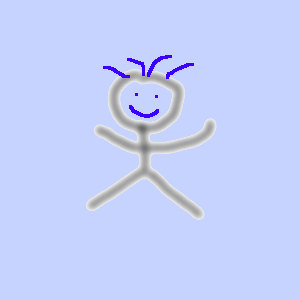
\includegraphics[keepaspectratio=true,scale=0.62]
    	{img/desenho.png}
    \fonte{do próprio autor.}
    \label{fig:desenhoAutor}
\end{figure}


\begin{table}[]
\centering
\caption{Exemplo de tabela}
\label{tab:exemploTabela}
\begin{tabular}{lll}
\toprule
Coluna 1                                              & Coluna 2            & Coluna 3 \\ \midrule
21		                                              & 21            		& 212 \\ 
11		                                              & 23            		& 32 \\ 
10		                                              & 11		            & 32 \\ \bottomrule
\end{tabular}
\fonte{Produzido pelos autores.}
\end{table}

As equações podem ser feitas ao longo do texto, por exemplo: $area = \frac{base \times altura}{2}$ ou apresentadas no ambiente \textit{equation}, como na Equação~\ref{eq:testeEquacao}.

\begin{equation}
	area = \frac{base \times altura}{2}
    \label{eq:testeEquacao}
\end{equation}

Finalmente, os textos possuem citações bibliográficas. A padronização das citações são apresentadas por~\citeonline{abntCitacoes2002}. A citação deve ser feita da seguinte forma: caso o nome do autor faça parte do texto, deve-se colocar entre parênteses apenas o ano. Por exemplo: \citeonline{brin1998anatomy} apresentaram o algoritmo PageRank. Caso contrário, o nome do autor ficará entre parênteses, em letras maiúsculas. Por exemplo: neste método foi utilizado o algoritmo Page Rank~\cite{brin1998anatomy,abntCitacoes2002}.


\section{Elementos Pós-textuais}
\label{sec:posTextual}

Os elementos pós-textuais são compostos das referências bibliográficas, do apêndice e dos anexos. A ABNT não estabelece um padrão para o título dessas seções. No presente documento, seguindo o template do ABNTex2, utilizou-se a fonte \textit{Latin Modern Sans} tamanho 24pt. Deverá haver numeração das páginas. Lembre-se: apêndice são materiais produzidos pelo autor do TCC enquanto anexo são materiais produzidos por outros autores. 
As normas de referências estão disponíveis em~\citeonline{abntCitacoes2002}\footnote{Neste site é possível verificar alguns exemplos: \url{http://www.leffa.pro.br/textos/abnt.htm}. Acesso em: 03 set. 2021.}. 

